%%%%%%%%%%%%%%%%%%%%%%%%%%%%%%%%%%%%%%%%%%%%%%%%%%%%%%%%%%%%%%%%%%%%%%%%
% RevTeX 4.1 LaTeX
% Kevin C. Young
% Scalable & Secure Systems Research (08961)
% Thu Mar  5 15:29:19 PST 2015
%%%%%%%%%%%%%%%%%%%%%%%%%%%%%%%%%%%%%%%%%%%%%%%%%%%%%%%%%%%%%%%%%%%%%%%%

\documentclass[aps,nofootinbib,pra,notitlepage,twocolumn]{revtex4-1}
\usepackage{amsfonts,amsmath,amssymb,amsthm}
 \usepackage{array,bm,color}
\usepackage{epsfig,graphicx,nomencl,revsymb4-1,upgreek,url}
\usepackage{hyperref}
\usepackage{algorithm}
\usepackage{algpseudocode}
\usepackage{graphicx}
\usepackage{calc}
\graphicspath{{./figures/}}
\hypersetup{colorlinks=true, pdfauthor=Kevin C. Young, pdftitle=Decorrelating Errors}
\newcommand{\tr}{{\rm Tr\thinspace}}
\newcommand{\bra}[1]{\ensuremath{\left\langle{#1}\right\vert}}
\newcommand{\ket}[1]{\ensuremath{\left\vert{#1}\right\rangle}}
\newcommand{\braket}[2]{\left\langle #1 | #2 \right\rangle}
\newcommand{\ketbra}[2]{\left| #1 \right\rangle\!\!\!\,\left\langle #2 \right|}
\newcommand{\abs}[1]{\left\vert #1 \right\vert}
\newcommand{\expect}[1]{\ensuremath{\left\langle{#1}\right\rangle}}
\newcommand{\timeorder}{\ensuremath{\underset{\leftarrow}{\mathcal{T}}}}
\newcommand{\ident}{{\mathbb1}}
\newcommand{\order}[1]{\mathcal{O}\left( #1 \right)}
\newcommand{\diag}[1]{\mathrm{diag}\{#1\}}
\newcommand{\trans}[1]{#1^\mathsf{T}}
\newcommand{\T}{\mathsf{T}}
\newcommand{\erf}[1]{Eq.~(\ref{#1})}
\newcommand{\needcite}{{\color{blue}\textsuperscript{[citation needed]}}}
\newcommand{\note}[1]{{\color{red}[#1]}}
\newcommand{\kcy}[1]{{\color{red}[#1]_{\rm{KCY}}}}
\newcommand{\amp}[1]{{\color{red}[#1]_{\rm{AMP}}}}
\newcommand{\deriv}[0]{{\frac{d}{d\vec{\delta}}}}
\newcommand{\actual}{\ensuremath{\tilde{\mathcal{G}}}}
\newcommand{\target}{\ensuremath{{\mathcal{G}}}}
\newcommand{\error}{\ensuremath{{\mathcal{E}}}}
\newcommand{\generator}{\ensuremath{{\mathsf{G}}}}
\def\id{\mbox{\small 1} \!\! \mbox{1}}

%-------------Header begins here----------------------------------------
\begin{document}
\title{Advantages of mixed quantum channels for information processing}

\author{Anthony M. Polloreno}
\email[Email: ]{anthony@rigetti.com}
\affiliation{Rigetti Computing, Berkeley, CA}

\author{Kevin C. Young}
\affiliation{Sandia National Laboratories, Livermore, CA}

\date{\today}

\begin{abstract}
Coherent errors in quantum operations are ubiquitous. Whether arising from spurious environmental couplings or errors in control fields, such errors can accumulate rapidly and degrade the performance of a quantum circuit significantly more than an average gate fidelity may indicate. As Hastings and Campbell have recently shown, randomly sampling an ensemble of implementations of a target gate yields an effective quantum channel that well-approximates the target, but with dramatically suppressed coherent error. Our results extend those of Hastings and Campbell to include robustness to drifting external control parameters. We implement these constructions using a superconducting qubit and will discuss randomized benchmarking results consistent with a marked reduction in coherent error.
\end{abstract}

\pacs{}

\maketitle


% ==============================================================================
% Section: Introduction
% ==============================================================================
\section{Introduction}
\label{sec:introduction}

The past decade has seen a dramatic increase in the performance and scale of quantum information processors (QIPs). Gate fidelities are now routinely in the 99\% to 99.99\% range \cite{Barends2014, Ballance2016, 1901.08035}, and dozens of individually-addressable qubits are becoming available on integrated devices. While these advances are promising steps forward on the path towards a computationally useful QIP, the quantum supremacy \cite{1203.5813} milestone has yet to be definitively reached. A critical limiting factor, of course, is errors in the quantum gate operations.

The ultimate impact of a gate error on a quantum circuit depends strongly on both the magnitude and the nature of the error. Systematic, or \emph{coherent}, errors can arise from poorly calibrated controls or imperfect gate compilations that induce repeatable, undesired unitary errors on the state of a QIP. Errors of this type are correlated in time may add up constructively or destructively, depending on the circuit. They are are  computationally expensive to model and it can be difficult to place tight analytic bounds on circuit performance [cite]. Contrast this against random, or \emph{stochastic}, errors, which often result from high-frequency noise in the controls or the environment. Systems with stochastic errors can usually be modeled by defining a rate of various discrete errors in the system, such as a bit flips or phase flips. These errors are significantly easier to simulate on a classical computer, and their impact on quantum circuits is much easier to estimate [Ken Brown, Steve Flammia].



\note{don't define diamond norm here}

Quantitative bounds on the performance of a quantum circuit composed of faulty gates can be constructed using the diamond distance, $||\cdot||_\diamond$. This particular metric, defined in Section \ref{sec:representing_quantum_gates}, has the appealing property of being subadditive, namely for a channels $\mathcal{F}_1$, $\mathcal{F}_2$ we have:
\begin{equation}
||\mathcal{F}_1\circ\mathcal{F}_2||_\diamond \leq ||\mathcal{F}_1||_\diamond + ||\mathcal{F}_2||_\diamond
\end{equation}
The diamond distance can be used to bound the total variation distance (TVD) of a quantum circuit, but it is in general sensitive at first order to repeated application of a gate with coherent errors. For long circuits, this can add up extremely quickly, and while these errors can often be identified and reconstructed using various tomographic techniques, their impact on a given quantum  difficult to predict. Additionally, despite the relative ease of modeling stochastic errors, coherent errors are often much more likely to appear in QIPs. Recent work by Campbell and Hastings\cite{Campbell2017, 1612.01011, 1811.08017}, however, has shown that coherent noise can be strongly suppressed by probabilistically mixing several distinct implementations of the target quantum gates. In this case, the resulting effective quantum process has a diamond distance that grows only quadratically in the over/under rotation angle of the component gates. 

\begin{figure}[t]
  \centering
  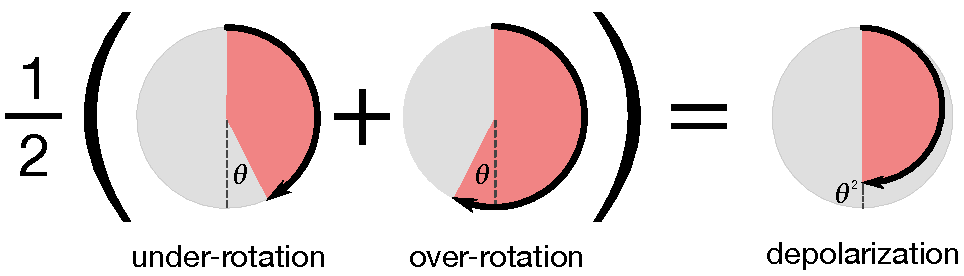
\includegraphics[width=\columnwidth]{simple_example.pdf}
  \caption{An example of a mixed quantum channel. Using optimal control, two implementations of a $Z_\pi$ gate are designed to have equal and opposite sensitivity to errors (if one implementation over-rotates by angle $\theta$, then the other \emph{under}-rotates by $\theta$). Each time the gate is used, one of these implementations is chosen at random. The resulting quantum channel is equivalent to a perfect implementation of the gate followed by dephasing of $\order{\theta^2}$.}
  \label{fig:simple_example}
\end{figure}

%Drifting control parameters or environmental variables can easily have long correlation times that result in errors which are strongly coherent over the length of a quantum circuit. 

In this article we discuss various applications of these mixed unitary controls, and show that the advantages of this approach can be made robust to drift in the gate implementations. We demonstrate that, depending on the objective, different numerical optimizations may be preferred. We present an experimental implementation of single-qubit mixed unitary controls on a superconducting qubit testbed at Rigetti Computing. Using randomized benchmarking, we are able to show a marked improvement in error rates, as well as a reduced variance in circuit outcome probabilities, indicating a reduction in the coherence of the error. We further provide an optimal control approach to the mixed unitary control design problem, and apply our methods in simulation where we construct single- and two-qubit mixed unitary controls which are robust to drift and uncertainty in the control parameters.   

% ==============================================================================
% Section: Mathematical preliminaries
% ==============================================================================
\section{Mixed quantum channels}
\label{sec:representing_quantum_gates}
\begin{enumerate}
	\item Specify the process matrix representation of a quantum channel in terms of the generalized Bloch vector
	\item 
\end{enumerate}
Quantum gate operations are implemented by applying a sequence of classical control fields to some set of qubits. Fluctuations in the environment or imperfections in the controls can cause the state of the qubits to change in a way that is different from what was intended.  But if the gates are fairly stable with time and context\cite{1810.05651}, then we can model their action with completely positive, trace-preserving (CPTP) maps. These maps have a number of useful representations, including as Kraus operators[], Choi matrices[], and Jamiolkowsi states[]. But for the purposes of this article, \emph{process matrices} will be most convenient. The process matrix representation of a quantum gate acts through the usual matrix multiplication on a vectorized representation of the system density matrix. \note{Write some more...}
\begin{equation}\label{error_def}
  \vec\rho \rightarrow \actual\vec\rho = \error \target \vec\rho.
\end{equation}
We vectorize the density matrix as
\begin{equation}
  \vec \rho = \tr(\rho \vec \Sigma)/2^n,
\end{equation}
where $\vec \Sigma$ is a vector of all $4^n$ $n$-qubit Pauli operators. For a single qubit, this is $\vec\Sigma = \left\{I, \sigma_x, \sigma_y, \sigma_z\right\}$.  We can then represent the action of a CPTP map using a \emph{process matrix}, which acts on a vectorized quantum state by the usual matrix multiplication:



An important consequence of the linearity of this representation is that classical randomness can be easily encoded in the density matrix. Suppose that each time a gate is implemented, a different version of the gate is applied at random. 

Here $\actual$ is the actual gate as implemented, $\target$ is the target operation, and $\error$ is the effective error channel:
\begin{equation}\label{eq:process_matrix}
\error =
	\left(\begin{array}{c|cccc}
		1 &  & \vec{0}^T & \\ 
		\hline & &  &  \\
		\vec{m} &  & R &  \\
		 &  &  & 
	\end{array} 	
	\right)
\end{equation}
The top row of all trace-preserving (TP) maps is fixed to $\{1,0,0,0,\cdots\}$.  The rest of the first column, $\vec{m}$, describes any deviations from unitality, as could arise from amplitude damping. If the error channel is unitary, then the error is coherent, and the submatrix $R$ is perfectly antisymmetric, corresponding to a rotation of the generalized Bloch vector. If  $R$ is diagonal, then the error channel is Pauli stochastic, with each entry  corresponding to the probability that the associated Pauli error occurs in each application of the gate. Any such Pauli error is expressible as a unitary matrix $U$ that acts on the density matrix by conjugation, and has an action on the vectorized density matrix given by: 
\begin{equation}
\vec{\rho}\rightarrow \rho_i\vec{\Sigma}_{ijk}U^{\dagger}_{kl}\vec{\Sigma}_{lmn}U_{mj}\end{equation}
 If R is symmetric but not diagonal, then the channel is still stochastic, but the random errors consist of correlated Pauli operators (such as $X+Y$). For a single qubit, this describes everything, but the situation can be slightly more complicated for more qubits. 

In addition to the type of errors, we care about the size of an error. The \emph{size} of an error in quantum gates may  be quantified in a number of ways. Two of the most common metrics are the average gate fidelity, $\mathcal{F}$, and the diamond norm, $\vert\vert\cdot\vert\vert_\diamond$. These may be represented in terms of the error maps as
\begin{align}
	&\vert\vert I - \error \vert\vert_\diamond = \sup_\rho \vert \vert (I\otimes I)(\rho) - (\error \otimes I)(\rho) \vert\vert_1\\
	&\mathcal{F}(\error) = \frac{\tr{\error} + d}{d^2 + d} 
\end{align}

Which metric is relevant depends on the application, and can yield very different numbers. For instance, the diamond norm is generally linear in the over-rotation angle of a quantum operation, while the average gate infidelity (AGI), given by 1-$\mathcal{F}$, is generally quadratic in the over-rotation angle of a quantum operation. These two metrics also vary significantly in performance on mixed processes.

A \textit{mixed quantum channel} (MQC) consists of a set of unitary channels, $\actual_j$, and associated weights, $\sum_j \omega_j = 1$.  The process matrix for a mixed unitary channel is then the weighted sum of the component channels, $\actual_{\rm M} = \sum_j \omega_j \actual_j$, and the associated error channel is simply the weighted sum of the associated error channels, $\error_{\rm M} = \sum_j \omega_j \error_j$. From this definition, we can use linearity to compute the AGI of a MQC. We see that the AGI of any MQC will be the convex sum of the consituent fidelities, with the same weighting. The diamond norm, however, is non-linear function of the channel, and can in general be smaller for a MQC than any of the processes being mixed. 

When performing a quantum gate, there are often many possible ways of it might be implemented. Campbell and Hastings, for instance, consider gates compiled using the Solovey-Kitaev algorithm, for which many approximate gate compilations are possible.\cite{Campbell2017, 1612.01011} Following this, Campbell considered the important problem of minimizing the diamond norm of the resulting error channel. Given a collection of component channels with error at most $\epsilon$, he showed that if the Hamiltonians form a convex set containing the origin, then the diamond norm can be quadratically supressed. The diamond norm is a particularly appealing target because the it provides useful error bounds on quantum circuits. However, it is not the only optimization target that can be chosen. 

\subsection{A simple example}
\label{sec:simple_example}
As a simple example, consider a scenario in which we have a single-qubit and four possible implementations of a $\pi$-pulse about the $\sigma_x$ axis. The error channels for these four implementations are themselves unitary rotations about the $\sigma_x$ axis with rotation angles of $\{-2\epsilon, -\epsilon, \epsilon, 2\epsilon\}$. Such a situation could appear, for instance, if there were amplitude errors on the fields used to affect the gates, and if the control could be implemented by a rotation about the positive or negative $\sigma_x$ axis.



In such a scenario, if the ultimate goal is to produce a channel whose effect can be Monte Carlo simulated, then a useful approach would be to construct a channel whose errors are Pauli stochastic. Such a channel could be constructed, for instance, by drawing from this collection uniformly at random. More generally, given a collection of control, such a channel could be produced by minimizing the off-diagonal elements of $R$ in Equation \ref{eq:process_matrix}. We implemented such a routine on a superconducting qubit.

The error operator corresponding to a rotation error by angle $\epsilon$ is then:
\begin{equation}
\error(\epsilon) =
	\left(\begin{array}{ccccc}
		1 & 0 & 0 & 0 \\ 
		0 & \cos\epsilon & \sin\epsilon  & 0  \\
		0 & -\sin\epsilon & \cos\epsilon & 0  \\
		0 & 0 & 0 & 1
	\end{array} 	
	\right)
\end{equation}

The associated diamond distance of this channel is $\abs{\mathcal{I} - \error(\epsilon)}_\diamond \simeq \epsilon$, while the fidelity of the channel is $\mathcal{F}(\error(\epsilon)) = \epsilon^2$. If we were construct two channels, one with error $\error(\epsilon)$ and one with error $\error(-\epsilon)$, then we could construct a new channel with error $\error_{\rm eff} = \frac{1}{2}\left(\error(\epsilon) + \error(\epsilon)\right)$. The effective channel then has a matrix representation:
\begin{equation}
	\error(\epsilon) =
	\left(\begin{array}{ccccc}
		1 & 0 & 0 & 0 \\ 
		0 & \cos\epsilon & 0  & 0  \\
		0 & 0 & \cos\epsilon & 0  \\
		0 & 0 & 0 & 1
	\end{array} 	
	\right) \simeq \mathcal{I} - 
	\left(\begin{array}{ccccc}
		0 & 0 & 0 & 0 \\ 
		0 & \epsilon^2/2 & 0  & 0  \\
		0 & 0 & \epsilon^2/2 & 0  \\
		0 & 0 & 0 & 0
	\end{array} 	
	\right)
\end{equation}
And with same average process fidelity, $\epsilon^2$, but now a suppressed diamond norm $\epsilon^2$. Now write this in terms of the error generators $\error(\epsilon) = \exp(\epsilon G)$ where
\begin{equation}
	G =
	\left(\begin{array}{ccccc}
		0 & 0 & 0 & 0 \\ 
		0 & 0 & -1  & 0  \\
		0 & 1 & 0 & 0  \\
		0 & 0 & 0 & 0
	\end{array} 	
	\right)
\end{equation}

The effective generator vanishes at first order.

\begin{equation}
	\error(\epsilon) = \mathcal{I} + \epsilon G + \frac{1}{2}\epsilon^2 G^2 + \mathcal{O}(\epsilon^3)
\end{equation}
\begin{align}
	\error_{\text{eff}} 
		% &= \sum_i \omega_i \error_i \\
		% &= \sum_i \omega_i \left(\mathcal{I} + \epsilon_i G_i + \frac{1}{2}\epsilon_i^2 G_i^2 + \cdots \right) \\
		&= \mathcal{I} + \sum_i \omega_i \epsilon_i G_i+ \sum_i \omega_i \frac{1}{2}\epsilon^2_i G_i^2 + + \mathcal{O}(\epsilon^3)
\end{align}
\begin{equation}
	\error_{\text{eff}} = \mathcal{I} + \sum_i \omega_i \frac{1}{2}\epsilon^2_i G_i^2 + \mathcal{O}(\epsilon^3)
\end{equation}

\begin{center}
\begin{tabular}{cccc}
	Gate & $H_{\rm{eff}}$ & AGI & $\vert\vert\cdot\vert\vert_\diamond$ \\
\hline
	$U_{+2\epsilon}$ & $2\epsilon \sigma_x$ & $4\epsilon^2$ & $2\epsilon$\\
	$U_{+\epsilon}$ & $\epsilon \sigma_x$ & $\epsilon^2$ & $\epsilon$ \\
	$U_{-\epsilon}$ & $-\epsilon \sigma_x$ & $\epsilon^2$ & $\epsilon$ \\
	$U_{-2\epsilon}$ & $-2\epsilon \sigma_x$ & $4\epsilon^2$ & $2\epsilon$ 
\end{tabular}
\end{center}

Alternatively, we might consider eliminating off-diagonal entries of $\error(\epsilon)$ \note{fix this}:
\begin{equation}
	\left(\begin{array}{@{}ccccc@{}}
		0 & 0 & 0 & 0 \\ 
  		\cline{3-4}
    	0 & 0 & \multicolumn{1}{|c}{-1} & \multicolumn{1}{c|}{0} \\
    	\cline{3-3}		
		0 & 1 & 0 & \multicolumn{1}{|c|}{0}\\
		\cline{4-4}	
		0 & 0 & 0 & 0
	\end{array} 	
	\right)
\end{equation}
 resulting in a matrix that is guaranteed to be Pauli stochastic, and thus somewhat easily simulable problem. In the case of a single qubit, it is clear that our generator is expressible as $\hat{n}\cdot\vec{\Sigma}$, where $\vec{\Sigma}$ is again the vector of Pauli operators. The condition that the off-diagonal terms vanish is then again the same condition that the origin lies in the convex hull of the vectors $\vec{n}_i$ for each $G_i$.
 \note{more here about alternative method. Also discuss Fig 2.}. 


\note{END}


% In general, if we have a collection of single qubit controls $\{U_i\}$ generated by $\{H_i\}$, the channel that results from drawing from the controls probabilistically has elements given by:
% \begin{align}
% 	\mathcal{M}_{jk} 
% 		=& \sum_i p_i \tr{(\sigma_j^{\dagger}U\sigma_kU^{\dagger})} \\
% 		=& \sum_i p_i \tr{(\sigma_j^{\dagger} \exp(i \frac{\theta_i}{2} H_i)\sigma_k		\exp(-i \frac{\theta_i}{2} H_i)}) \\
% 		=& \tr (\sum_i p_i (\sigma_j^{\dagger}\sigma_k\cos\theta_i^2 + \sigma_j^{\dagger}H_i\sigma_k H_i\sin\theta_i^2 \\ 
% 		&+ i\sigma_j^{\dagger}H_i\sigma_k\sin\theta_i\cos\theta_i - i\sigma_j^{\dagger}\sigma_kH_i\sin\theta_i\cos\theta_i))
% \end{align}
% The first term corresponds to the identity, and $\sin\theta_i^2$ is always positive, so we cannot hope to eliminate the second term, but $\sin\theta_i\cos\theta_i$ may be positive or negative, and so there is hope that we could possibly combine various implementations to eliminate this term. The result would be a purely stochastic channel. 

\begin{figure}
  \centering
  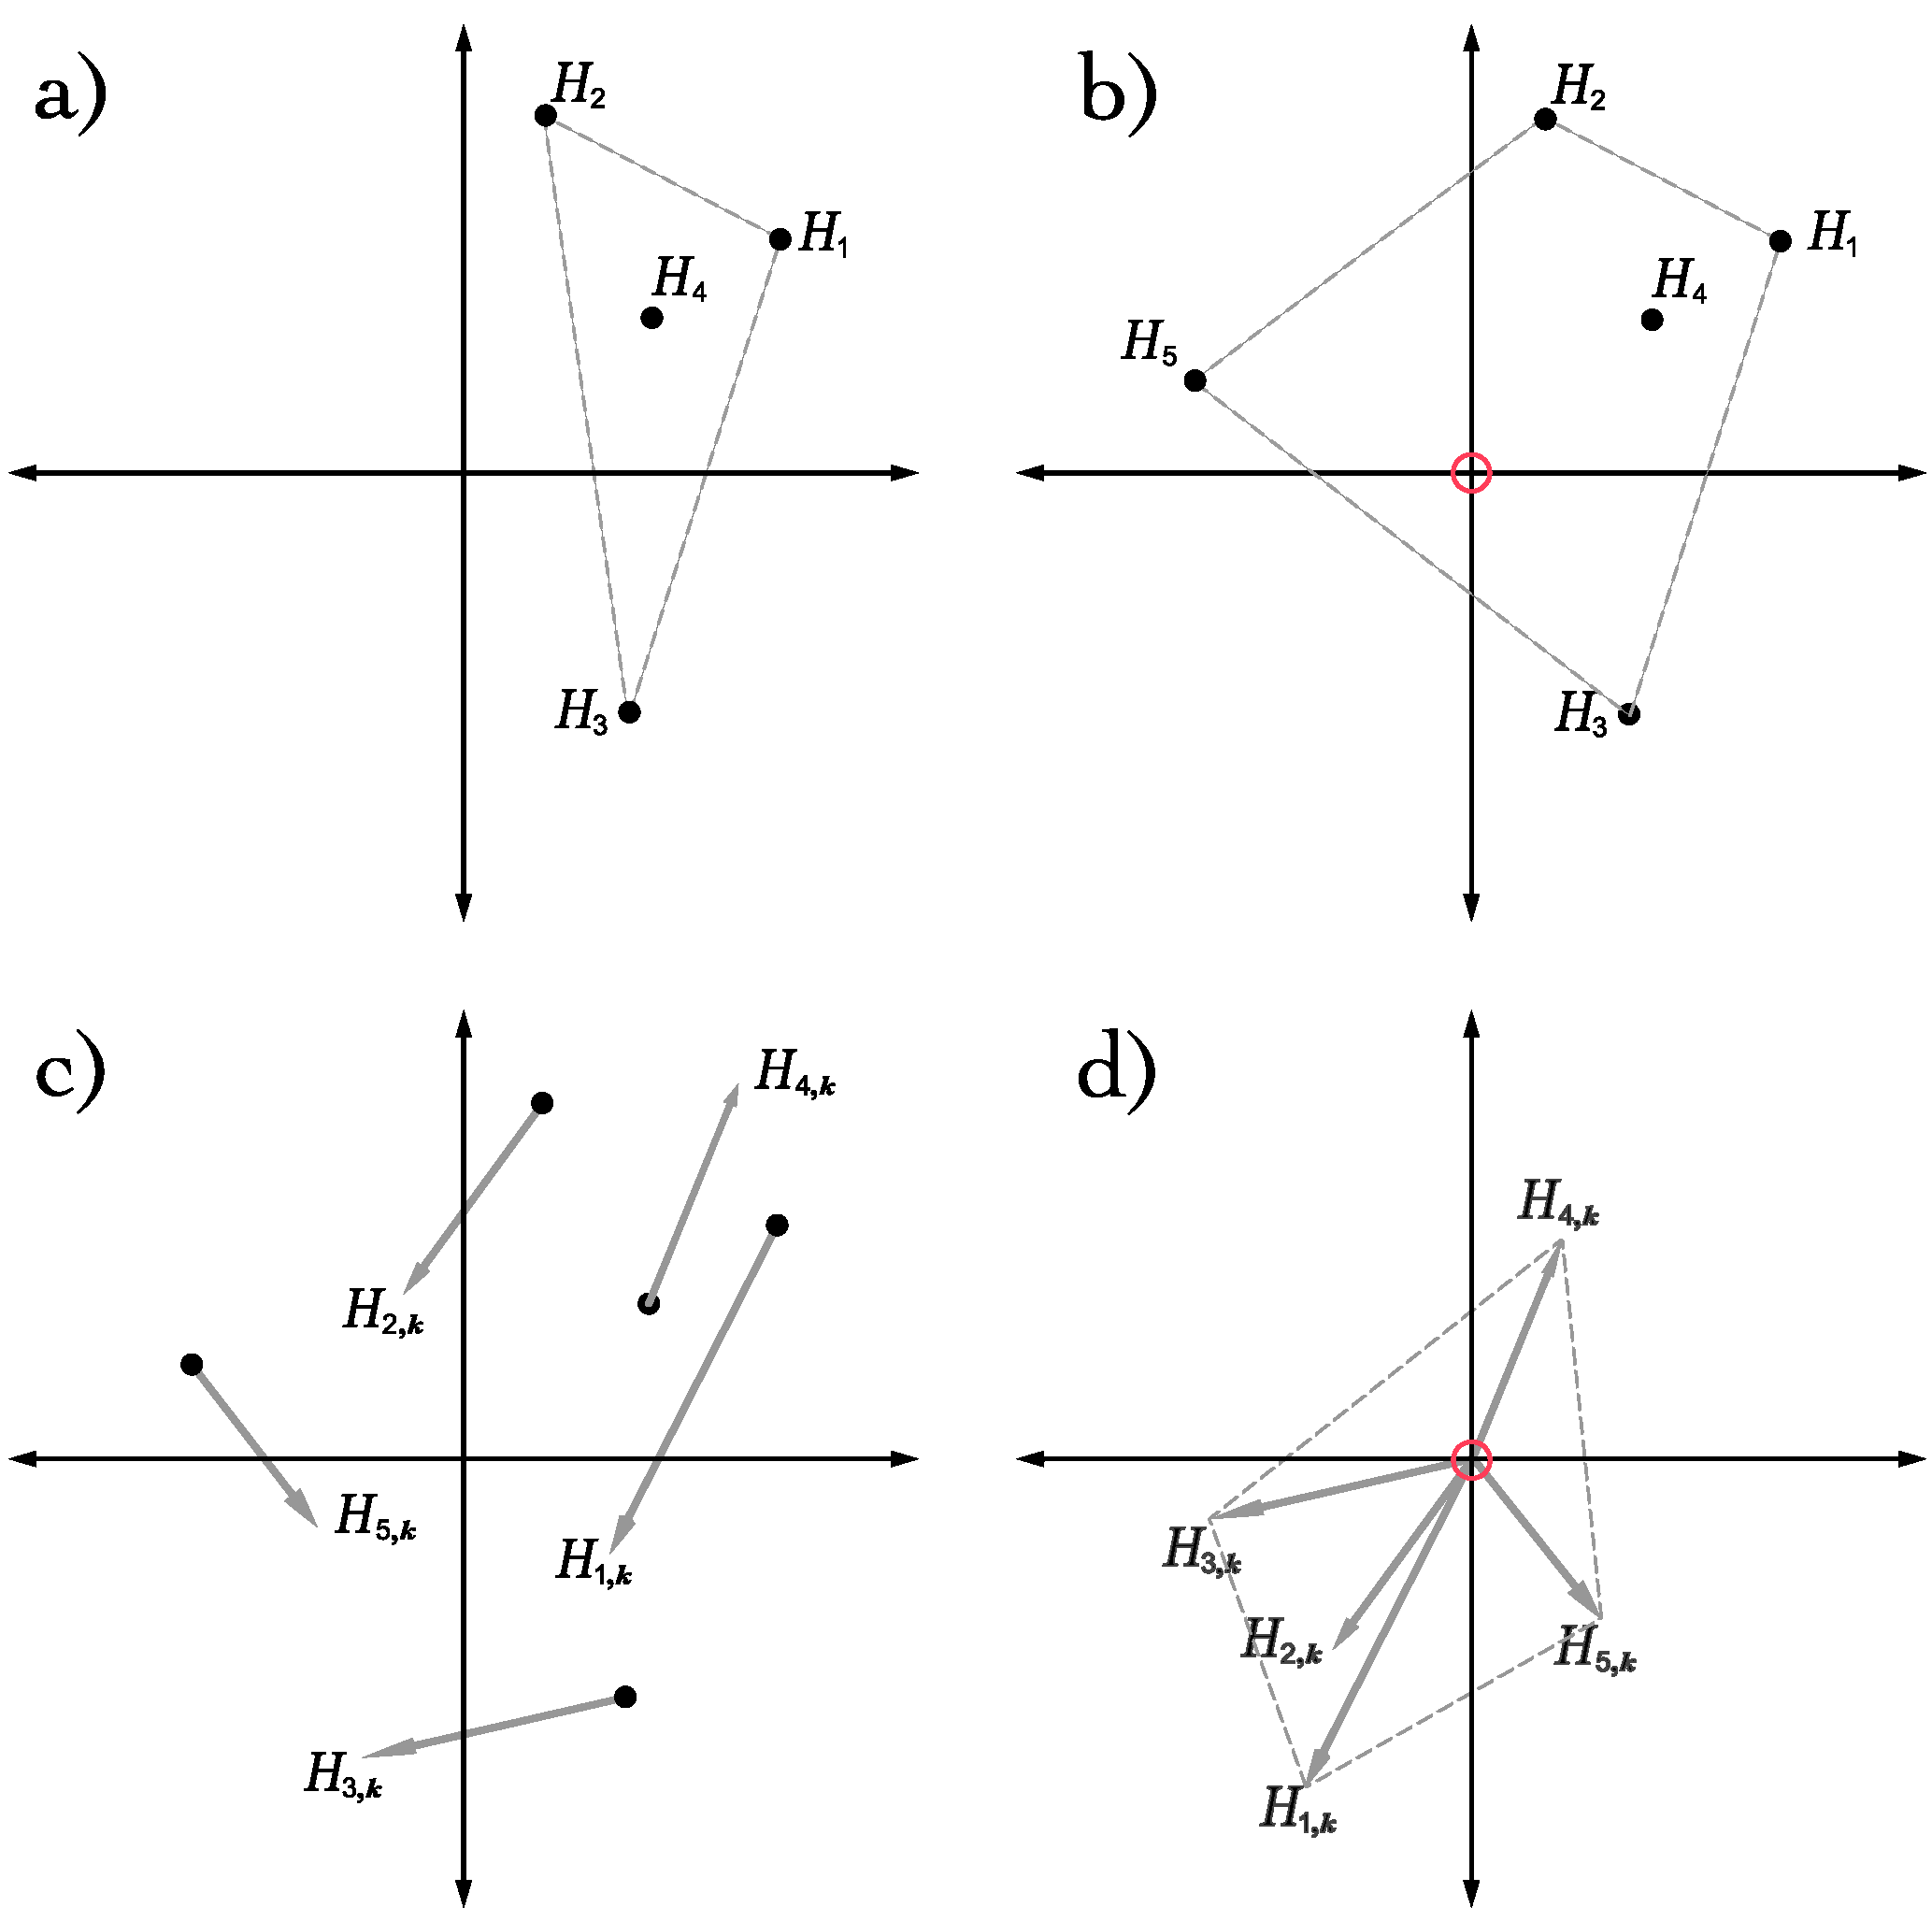
\includegraphics[width=\columnwidth]{vectorspace.pdf}
  \caption{A target unitary gate can be implemented a number of ways, each with a different effective Hamiltonian error. These error Hamiltonians lie in a vector space. a) Four effective Hamiltonians. The origin is not contained in their convex hull, so there are no 0MQCs. b) The origin is contained in the covex hull after adding an additional control solution. Because there are more than $n+1$ implementations, there exist an infinite number of 0MQCs. c) The error Hamiltonians shown with their derivative with respect to a control parameter. As this parameter drifts, a 0MQC may drift, leading to a first-order error. d) The derivatives also lie in a vector space. If the origin lies in their convex hull, then it may be possible to construct a 1MQC.}
  \label{fig:vectorspace}
\end{figure}

% The problem of minimizing the last term:
% \begin{equation}
% \sum_i\sin\theta_i\cos\theta_i(\sigma_j^{\dagger}H_i\sigma_k - \sigma_j^{\dagger}\sigma_kH_i)
% \end{equation}
%  can equivalently be cast as trying to construct a family of vectors whose convex hull contains the origin. This can be seen in Figure \ref{fig:vectorspace} a) and b).



% ==============================================================================
% Section: Constructing Useful Mixed Quantum Channels
% ==============================================================================
\section{Constructing Useful Mixed Quantum Channels}
\label{sec:mixed_unitary_processes}
Motivated by the simple example provided in Section \ref{sec:simple_example}, we would like to find a general methodology for producing \textit{useful} mixed quantum channels. In each of the optimization targets we considered, the problem reduces to finding a collection of vectors whose convex hull contains the origin. These vectors might represent a collection of error generators or the off-diagonal elements of a collection of error maps. As we'll see in Section \ref{sub:adding_robustness}, we can also consider the derivates of the error generators, if we want to consider the sensitivity of the controls to drift. By considering the appropriate collection of vectors and weightings, we can minimize any number of effects. Which routine we choose will depend on the quantities we are trying to minimize.

% ==============================================================================
% Section: Generators
% ==============================================================================
\subsection{Optimization Targets}
\subsubsection{First-order generators} % (fold)
\label{sub:first_order_generators}
If our primary goal is for our MQC to have increased performance, then a useful target for constructing MQCs is to minimize the diamond norm. The diamond norm is a non-linear function that in general requires a convex optimizer to compute. However, if our errors are small enough, we can consider the linearized problem, and minimize the diamond norm to first-order. As in Section \ref{sec:simple_example}, the MQC that minimizes the diamond norm to first-order in $\epsilon$ is:
\begin{equation}\label{eq:balanced}
\mathcal{M}_{jk} = \frac{1}{2}\tr(\sigma_j^{\dagger}U_{-\epsilon}\sigma_kU_{-\epsilon}^{\dagger}) + \frac{1}{2}\tr(\sigma_j^{\dagger}U_{\epsilon}\sigma_kU_{\epsilon}^{\dagger})
\end{equation}
This channel will have a diamond norm proportional to $\epsilon^2$, whereas any other combination will have a linear dependence on $\epsilon$. Contrast this with the fact that any linear combination of $\{U_{\epsilon}, U_{-\epsilon}\}$ minimizes the AGI of the resulting channel with a value of $\epsilon^2$. While selecting the convex mixture of unitaries that minimizes the AGI is  trivial, the problem of efficiently minimizing the diamond norm can be difficult, and may be the relevant quantity to consider depending on the application. However, as discussed in \cite{Campbell2017}, a sufficient condition to minimize the diamond norm of a MQC with error generators $\{G_j\}$ to first order is:
\begin{equation}\label{eq:campbell-condition}
\sum \omega_j G_j = 0
\end{equation}
In \cite{Campbell2017} Campbell constructs an algorithm that, given an oracle to approximate unitaries, generates controls and weightings to find an MQC with this property. Alternatively one might ask the question: \textit{Given a fixed collection of controls, how can I produce weighting a weighting with minimal diamond norm?} Such a situation may arise if there is a natural family of controls that implement a desired gate, or if, as we consider later (Section \ref{sec:numerical_results}), we randomly generate a collection of gate implementations. In these situations, one can equivantly use convex optimization to solve this problem. Consider the matrix whose columns are the vectorized Hamiltonians at our disposal, i.e. for $m$, $n\times n$ Hamiltonians:
\begin{equation}\label{eq:vectorized_hamiltonians}
	\bold{G} = \left(\begin{array}{cccc}
		G_{1_{11}} & G_{2_{11}} & \ldots   \\ 
		\vdots\ & \ddots &    \\
		G_{1_{nn}} &  &  G_{m_{nn}} \\ 
	\end{array} 	
	\right)
\end{equation}
If our weighting vector for our MQC is $\omega$, we can rewrite this sum as a matrix product whose two-norm will be zero if and only if the sum is zero. Additionally, this optimization needs to be constrained so that $\omega$ only contains positive values that sum to one. This forms a convex optimization problem, and can be written as:

\begin{equation}\label{eq:minimization}
  \begin{split}
    &\underset{\omega_j\geq0, |\omega|_1=1}{\textbf{minimize}: } ||\bold{G}\omega||_2\\
  \end{split}
\end{equation}

Linearly constrained minimization problems with quadratic cost functions like this have been proven to be efficiently solvable by methods like the Elipsoid Method\cite{wright1999numerical, khachiyan}, and there are many existing convex solver software packages that solve these problems efficiently in practice, with some formal proofs showing runtimes as good as $\mathcal{O}(\log{\frac{1}{\epsilon}}L^2n^4)$, where $\epsilon$ is the accuracy in the solution, $L$ is the number of bits in the input, and $n^4$ is the number of variables.

%In both cases it is clear that we should select the gates with smaller error, i.e. $\{U_{\epsilon}, U_{-\epsilon}\}$, rather than those with larger error, to minimize the multiplicative coefficient on the error. Despite this, literature commonly assumes that all controls are less than some threshold value, below which differences in performance don't matter. \cite{Campbell2017} In realistic scenarios, some controls will have better performance than others, and it is important to select from those controls when able to. We will discuss numerical approaches to solving this Section \ref{sec:norm}.

%Another interesting property of the MQC given in Equation \ref{eq:balanced} is that it maintains its first-order insensitivity even in the presence of drift. In particular, if the control amplitudes that implement these gates drift, they will drift in equal and opposite ways. Thus, the resulting depolarizing channel (see Figure \ref{fig:simple_example}) will have a time-dependent strength, but it will remain first-order insensitivity to the static detuning $\epsilon$. In Section \ref{sec:robustly_mixed} we will provide a method for producing controls that exhibit this robustness to drift to arbitrary order. Given these considerations from this simple example, we will now consider a numerical strategy for generating MQCs.


% subsection first_order_generators (end)

% ==============================================================================
% Section: Off-diagonals
% ==============================================================================

\subsubsection{Off-diagonals} % (fold)
\label{sub:off_diagonals}
Instead of targeting the diamond norm and vectorizing the error generators, we can instead consider error channels $\error_i$ such that $\error_i\actual_i=\target$, where $\target$ is again the target gate. To approximate a depolarizing channel we may define a different minimization problem to  minimize the off-diagonal terms:
\begin{equation}\label{eq:minimization}
  \begin{split}
    &\underset{w_0, ..., w_N}{\textbf{minimize}} \{\sum_{i\neq j}^N|\sigma_i\Lambda(\sigma_j)|^2\}\\
    &\textbf{where}\ \Lambda(\sigma_j) := \sum^N_{i=1}w_i\mathcal{E}_i^{\dagger}\sigma_j\mathcal{E}_i\\
    &\textbf{subject to} \sum_{i=1}^Nw_i = 1
  \end{split}
\end{equation}

Previous authors have considered minimizing the diamond distance to the nearest Pauli or Clifford Channel \cite{Magesan2013}, and while this gives a good theoretical framework, it requires the use of a convex solver, and in particular does not have the restriction that the optimal channel be decomposable into a given family of controls. Therefore we can view our approach as a regularization of this method, where we have imposed the condition that our final channel must arise from a BCS. In doing so, we move from computing the diamond norm to needing to computing a sum. In the next section we give a simple example, followed by numerical results for one qubit and two qubits gates.
% subsection off_diagonals (end)

% ==============================================================================
% Section: Robustness
% ==============================================================================
\subsection{Additional Constraints}
\subsubsection{Adding robustness} % (fold)
\label{sub:adding_robustness}
\note{ Try to make this more readable }
While mixed quantum channels offer significant improvements to gate performance, they fail to take into account the reality that most control electronics experience drift over time scales relevant to QIP performance. Because of this drift, the quality of the MQC will degrade. Thus, we would like to design MQCs that are \textit{robust} to this drift. To enforce robustness, we can consider higher derivatives of the generators in Equation \ref{eq:campbell-condition}. Instead of only requiring that the $0^{th}$-order derivatives average to zero, we will impose a similar condition on the higher-order derivatives with respect to parameters that may drift:
\begin{equation}
D^n_j = \frac{1}{n!}\frac{\partial^{n}}{\partial\delta_{i_1}\ldots\partial\delta_{i_n}}H_j(\vec{\delta})|_{\delta=\vec{0}}
\end{equation}
If the dimension of $\vec{\delta}$ is $d$, the indices $i_0, \ldots, i_n$ take on values in $1, \ldots, d$ and this matrix has $d^n$ entries. 
We say that a mixed quantum channel is robust to order $\ell$ (an $\ell$MQC) if for all $1 \leq k \leq \ell$:
\begin{equation}\label{eq:MQC}
\begin{gathered}
\sum_j\omega_j(\sum_{n=0}^k D^n_j)^n = \vec{0}\\
\end{gathered}
\end{equation}
In particular, we see that a 0MQC satisfies Equation \ref{eq:campbell-condition}. More generally, these conditions imply that an $\ell$MQC is insensitive to the $\ell^{th}$ order in drift in $\vec{\delta}$. To see this, we can rewrite the error on each control in the MQC as:
\begin{equation}\label{eq:taylor}
\begin{gathered}
\actual_j(\vec{\delta}) = \exp(-i(H_j(\vec{0}) + \frac{\partial}{\partial\delta_i}H_j(d\delta_i)\\ +  \frac{1}{2}\frac{\partial^2}{\partial\delta_i\partial\delta_k} H_j(d\delta_i d\delta_k) + \ldots))\target
\end{gathered}
\end{equation}
By Taylor expanding Equation \ref{eq:taylor} in $\vec{\delta}$, one finds that the the first $\ell$ derivatives of an $\ell$MQC will be zero. Furthermore, if we are only interested in being first order insensitve to drift and can find controls such that $|D_j^n|\approx\epsilon$, we can approximate Equation \ref{eq:MQC} as:
\begin{equation}\label{eq:MQC-relaxed}
\begin{gathered}
\sum\omega_jD^n_j = 0\\
\end{gathered}
\end{equation}
This condition guarantees that errors will be supressed quadratically for all derivatives up to order $\ell$. A proof is included in the appendix that generalizes the Hastings-Campbell Mixing Lemma in \cite{Campbell2017}. Namely, Campbell showed that if $0\in $ Conv$[\{H_i(\vec{\delta})\}]$, where Conv is the convex hull of its arguments, then an $\vec{\omega}$ exists that quadratically decreases the diamond norm. We prove that $0\in $ Conv$[\{D_j^n(\vec{\delta})\}]$ implies there is an $\vec{\omega}$ exists that quadratically decreases the $\ell^{th}$-order sensitivity of the diamond norm of an $\ell$MQC. Figure \ref{fig:vectorspace} gives geometric intuition for the conditions required to produce an $\ell$MQC.

To generate robustly mixed quantum channels, we first define the vectorized derivative matrix ${D^{\ell}}$ in a similar way to Equation \ref{eq:vectorized_hamiltonians}:
\begin{equation}
{\bold{D}^{\ell}} =  \left(\begin{array}{cccc}
		D^\ell_{1_{11}} & D^\ell_{2_{21}} & \ldots   \\ 
		\vdots\ & \ddots &    \\
		D^\ell_{m_{11}} &  &  D^\ell_{m_{nn}} \\ 
	\end{array} 	
	\right)
\end{equation}

Using this, we can then solve the following convex optimization problem, generalizing Equation \ref{eq:minimization}:

\begin{equation}\label{eq:robust_minimization}
  \begin{split}
    &\underset{\omega_j\geq0, |\omega|_1=1}{\textbf{minimize}: } ||{\bold{D}^{\ell}}^T\omega||\\
    &\textbf{subject to: } \forall n<\ell, \sum \omega_jD_j^n=\vec{0}\\
  \end{split}
\end{equation}
with $D_n^j$ defined in Equation \ref{eq:taylor}. The time to solve these convex optimization problems is independent of the number of rows, which in our case is the number of drifting parameters. However, the size of the matrix that must be computed before solving grows as $Nd^{\ell}$, and the runtime of solving the optimization problem grows as $N^4$, with $d$ being the number of drifting parameters, and $N$ being the number of controls.

% subsection adding_robustness (end)

% ==============================================================================
% Section: Norm regularization
% ==============================================================================

\subsubsection{Hamiltonian Norm Regularization}
\label{sec:norm}
While up until this point, these particular convex optimization problem could be solved using a system of linear equations, casting them as convex optimization problems allows us to penalize the cost function to encourage different behavior in the solution. In particular, while this minimization problem is sufficient for quadratically decreasing the diamond norm relative to the \textit{worst} controls in the collection, it does not preferentially select the controls with the least error. That is to say, both \{$U_{+2\epsilon}$, $U_{-2\epsilon}$\} and \{$U_{\epsilon}$, $U_{-\epsilon}$\} from Section \ref{sec:simple_example} satisfy Equation \ref{eq:minimization}. To encourage the inclusion of controls with smaller error, we may impose a penalty proportional to the norm of the included Hamiltonians. In our case, we choose to penalize for the $\ell_2$ ($||\cdot||_2$) norm, and thus we modify our cost function to be:

\newcommand{\bunderbrace}[2]{%
  \begin{array}[t]{@{}c@{}}
  #1\\
  \parbox{\widthof{#1}}{$\scriptscriptstyle#2$}
  \end{array}
}

\begin{equation}\label{eq:minimization_l2}
\begin{split}
&\underset{n\in[N]}{\textbf{minimize}}\{\\
&\ \ \bunderbrace{\textbf{minimize}: }{\omega_j\geq0, |\omega|_1=1} ||{\bold{D}^{\ell}}^T\omega||+ \eta\sum\omega_j||D^0_j||_2\\
&\ \ \textbf{subject to: } \forall n<\ell, \sum \omega_jD_j^n=0\\
&\}
\end{split}
\end{equation}
with $\eta \geq 0$. By making $\eta$ larger, we can supress the diamond norm to second order, while ensuring that we are selecting those that will give us a smaller prefactor. The absolute value of $\eta$ depends on the particular numerical values in $\bold{D}^\ell$. Naively generating the 1Q 0MQC in the previous section results in nontrivial support on all the members of the control family. However, by rewriting the minimization to impose this sparsity constraint discussed in Section \ref{sec:robustly_mixed}, the resulting 0MQC uses just five of the controls. This shows that through adding constraints to our optimization routine, we can make the MQC practically useful. 


% ==============================================================================
% Section: Sparsity
% ==============================================================================

\subsubsection{Sparsity Constraints}
As a practical consideration, we would also like to regularize our objective function to enforce sparsity. Control electronics often have a limited amount of waveform memory, and thus it is important that MQCs have non-trivial probability support on a small number of controls. As an example of where this would be necessary is given in Figure \ref{fig:vectorspace}. In b), it is clear that $H_4$ is unecessary to contain the origin in the convex hull of the error generators. Thus we would prefer that our solution, if we are forming a $0$MQC, ignores $H_4$. However, if we additionally want our controls to form a 1MQC, we see from Subfigure D that we need $H_4$ in our control set, in which case we would like our algorithm to exclude $H_1$, since its derivative is contained in the convex hull of the others'. Thus we would like to be frugal in which controls we select. In many machine learning contexts, lasso regularization \cite{tibshirani1996regression} can be used to enforce sparsity in solutions, however this is insufficient in this context as we already constrain the one norm of $\omega$ to be one. Conveniently, the problem of enforcing sparsity in such situations has been considered in \cite{NIPS2012_4504} and can be expressed via another convex program that extends Equation \ref{eq:minimization}:

\begin{equation}\label{eq:minimization_regularization}
\begin{split}
&\underset{n\in[N]}{\textbf{minimize}}\{\\
&\ \ \bunderbrace{\textbf{minimize}: }{\omega_j\geq0, |\omega|_1=1,\\ t\geq0} ||{\bold{D}^{\ell}}^T\omega|| + t\\
&\ \ \textbf{subject to: } \omega_n > \frac{\lambda}{t}\\
&\ \ \phantom{\textbf{subject to: }} \forall n<\ell, \sum \omega_jD_j^n=0\\
&\}
\end{split}
\end{equation} with $\lambda\geq0$. As with $\eta$ in the last subsection, the optimal value of this parameter is problem specific, depending on $\bold{D}^\ell$, and how sparse the solution needs to be. For $\lambda$ small, the problem reduces to the original problem, and for $\lambda$ large we see that if $\omega$ is not sparse then $t$ must be very large, which increases the cost of that particular solution.
In both the 0MQC and the 1MQC case in our numerical implementation we imposed the same $\ell_2$ penalty, so that the algorithm preferentially selects controls with smaller errors. Adding this constrain made the 0MQC perform better at the origin by nearly an order of magnitude, and moved the 1MQC from being out-performed by the 0MQC for all detunings, to out performing by nearly an order of magnitude when there is $.1\%$ drift in the controls. Imposing this constraint allows us to trade off flatness at the origin for performance.

\section{Results} % (fold)
\label{sec:results}

% ==============================================================================
% Section: Experimental Results
% ==============================================================================

\subsection{Experimental} % (fold)
\label{sub:experimental}
Here we present experimental results from implementing this routine on a fixed-frequency superconducting transmon qubit. In particular, we used qubit 8 on the Rigetti 19Q-Acorn chip, whose characterization can be found in \cite{1712.05771}. To implement a MQC on this qubit, four incorrectly calibrated Gaussian pulses were produced by scaling the pulseshape amplitude for a calibrated 10 sample 50ns $RX(\frac{\pi}{2})$ pulse by $106.4\%$,  $103.9\%$, $93.7\%$ and $91.2\%$.

As discussed in the previous section, we chose here to minimize the off diagonal elements of the process matrix. To benchmark the quality of the MQC, we then performed six randomized benchmarking experiments\cite{Magesan2011}: one for each over-- and under--calibrated pulse, one for the calibrated pulse, and one for the mixed process. We used $1000$ shots per experiment, $10$ sequences per sequence length, for sequence lengths of $2, 4, 8, 16, 32$ and $64$. In each case, our Clifford operations were decomposed into RX($\frac{\pi}{2})$) and RY($\frac{\pi}{2})$) pulses. In our implementation, these gates are implemented using the same pulse envelope definitions and control electronics, phase shifted by $\frac{\pi}{2}$ radians, and are therefore subject to identical miscalibration errors. The results are shown in Figure \ref{fig:rb} for sequence lengths $L=64$. Fitting to the randomized benchmarking decay curves, we find one-qubit gate fidelities of $99.3\%$ for the calibrated pulse, $98.9\%$ for Pulse1, $99.1\%$ for Pulse2, $98.9\%$ for Pulse3, $98.5\%$ for Pulse4, and $99.2\%$ for the MQC, demonstrating that it performs almost as well as the calibrated pulse, and better than the constituent pulses. 
\begin{figure}[t]
  \centering
  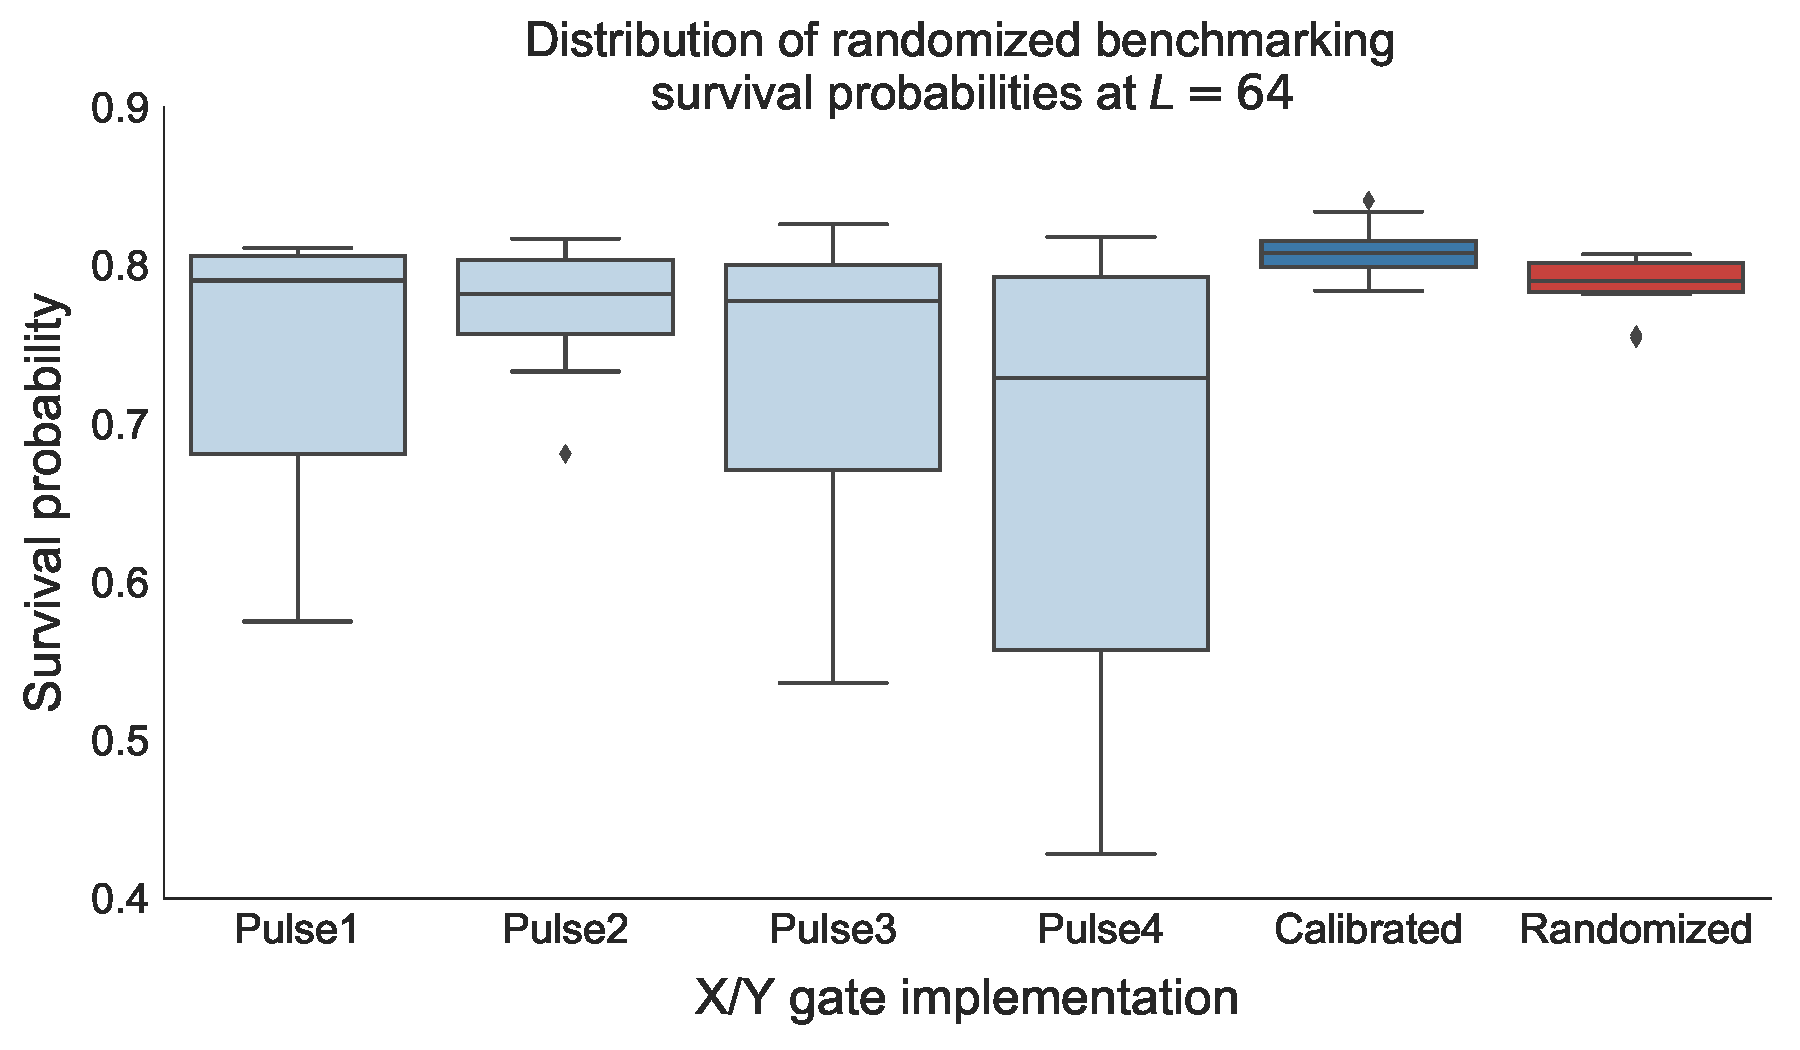
\includegraphics[width=\columnwidth]{rb_data.pdf}
  \caption{Randomized benchmarking experiments ran using different pulse definitions. The first four boxes result from using each of four different implementations of the ${\pi/2}$ rotations. The coherent noise present in these implementations leads to large variance of the survival probability over sequences. The fifth (dark blue) box illustrates the survival probability using a highly-tuned gate implementation. It displays improved average survival probability as well as reduced variance. The final box (dark red) illustrates the distribution over survival probabilities for a randomized MQC composed of Pulse1 through Pulse4. It performs comparably to the highly-calibrated implementation in both average survival probability and variance over random sequences. The reduced variance of the MQC is a tell-tale sign of reduced coherent error in the effective channel. }
  \label{fig:rb}
\end{figure}

Additionally, by minimizing the off-diagonal elements of the process matrix, we expect to produce a process with minimal coherent error. To see that this is the case, we cite the results in \cite{Ball2016}. For non-Markovian error models, noise will manifest as gamma distributed points for each sequence length. On the other hand, Markovian noise, such as depolarizing noise, will result in Gaussian distributed fidelity estimates for each randomized benchmarking sequence length. We see that the coherently miscalibrated controls in our RB experiment have long tails, consistent with gamma distributed random variables, while the calibrated and randomized implementations both have much shorter tails, consistent with Gaussian distributed random variables. Thus, our experiment demonstrates that not only is the performance of the MQC better than the constituent gates, it also has a signicantly less-coherent error channel.
% subsection experimental (end)


% ==============================================================================
% Section: Numerical Results
% ==============================================================================
\subsection{Numerical Implementation}
\label{sec:numerical_results}
In the following numerical results, we explore using the methods in Section \ref{sec:mixed_unitary_processes} to build MQCs. We consider the following model for a single tunable qubit: 
\begin{equation}\label{eq:1Qham}
  H(\delta, \epsilon, t) = \epsilon\sigma_z + (1 + \delta)(c_x(t)\sigma_x + c_y(t)\sigma_y)
\end{equation}
We use the GRAPE algorithm\cite{Khaneja2005} with N=25 steps and total evolution time of $\pi$ to generate 100 candidate controls. In our implementation, we modify the gradient so that we find controls that perform well in a Gaussian weighted neighborhood, with a standard deviation of $\sigma=.001$. We assume that the errors on $\sigma_x$ and $\sigma_y$ are perfecly correlated, as is the case in systems that implement RZ rotations with phase shifts of the control signal. Solving the optimization problem defined in Section \ref{sec:robustly_mixed} yields similar MQCs for $RX(\frac{\pi}{2})$ and $RY(\frac{\pi}{2})$, with the results for $RY(\frac{\pi}{2})$ shown in Figure \ref{fig:YMQC}. These results demonstrate several properties that make MQCs both useful and tractable.

\begin{figure}
  \centering
  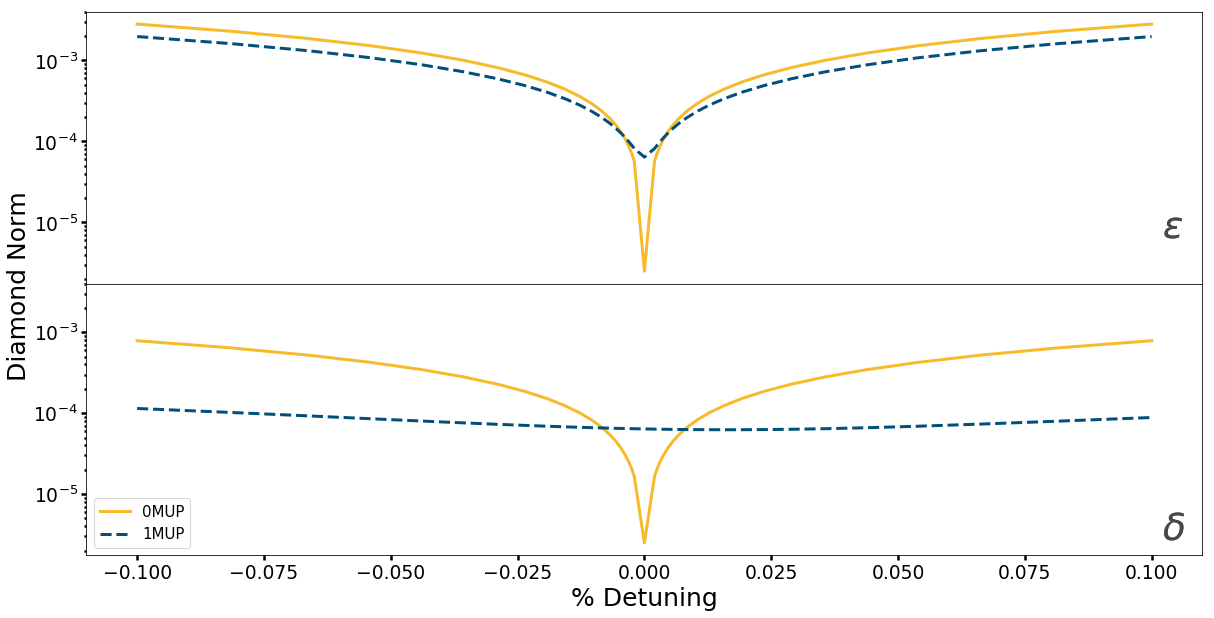
\includegraphics[width=\columnwidth]{SQRTY_no_member.png}
  \caption{Numerical results comparing a 0MQC to a 1MQC for a single tunable qubit, for $RY(\frac{\pi}{2})$. The results are qualitatively similar to those for $RX(\frac{\pi}{2})$. In this case the 0MQC outperforms both the 1MQC by two orders of magnitude, and the constituent controls by three orders of magnitude at the origin. However, varying over $\delta$ we see that the 1MQC outperforms the 0MQC by up to an order of magnitude when there is $.1\%$ drift in the qubit control amplitudes.}
  \label{fig:YMQC}
\end{figure}

In our two-qubit example we consider the following model for two tunable qubits coupled by a resonant exchange interaction, similar to that in \cite{McKay2016}:
\begin{equation} \label{eq:2Qham}
\begin{split}
H(\vec{\delta}, \vec{\epsilon}, t) = &\sum_{j=1}^2(\epsilon_j\sigma_z^j + (1 + \delta_j)(c_x^jx(t)\sigma_x^j + c_y^j(t)\sigma_y^j)) \\
&+ \frac{1}{10}(XX + YY)
\end{split}
\end{equation}

In this example it was infeasible to use GRAPE to return non-trivial solutions. Instead we manually selected piecewise constant echoing sequences with 500 steps and total evolution time of $\frac{5\pi}{2}$. In particular, we considered $RX(\pi)$, $RX(-\pi)$, $RY(\pi)$ and $RY(-\pi)$ bang-bang sequences \cite{bangbang}, consisting of all combinations of simultaneous $\pi$ pulses activated at multiples of $8$ steps from the beginning of the controls, and the same multiple of $8$ steps prior to the end of the controls. To give the control family a variety of RF errors, we added on uniformly distributed errors to each $\pi$ pulse, between $-.25$\% and $.25$\%.

In this example, we find more modest improvements to performance, as shown in Figure \ref{fig:2MQC}. There are now four free parameters to optimize over, and the uncontrolled entangling interaction means that there is little room for variation in the controls. Nonetheless, using a MQC improves performance by half of an order of magnitude at the origin relative to the constituent controls, and up to an order of magnitude away from the origin. For all values of the drifting parameters we see that the 1MQC performs as well or better than 0MQC.

\begin{figure}
  \centering
  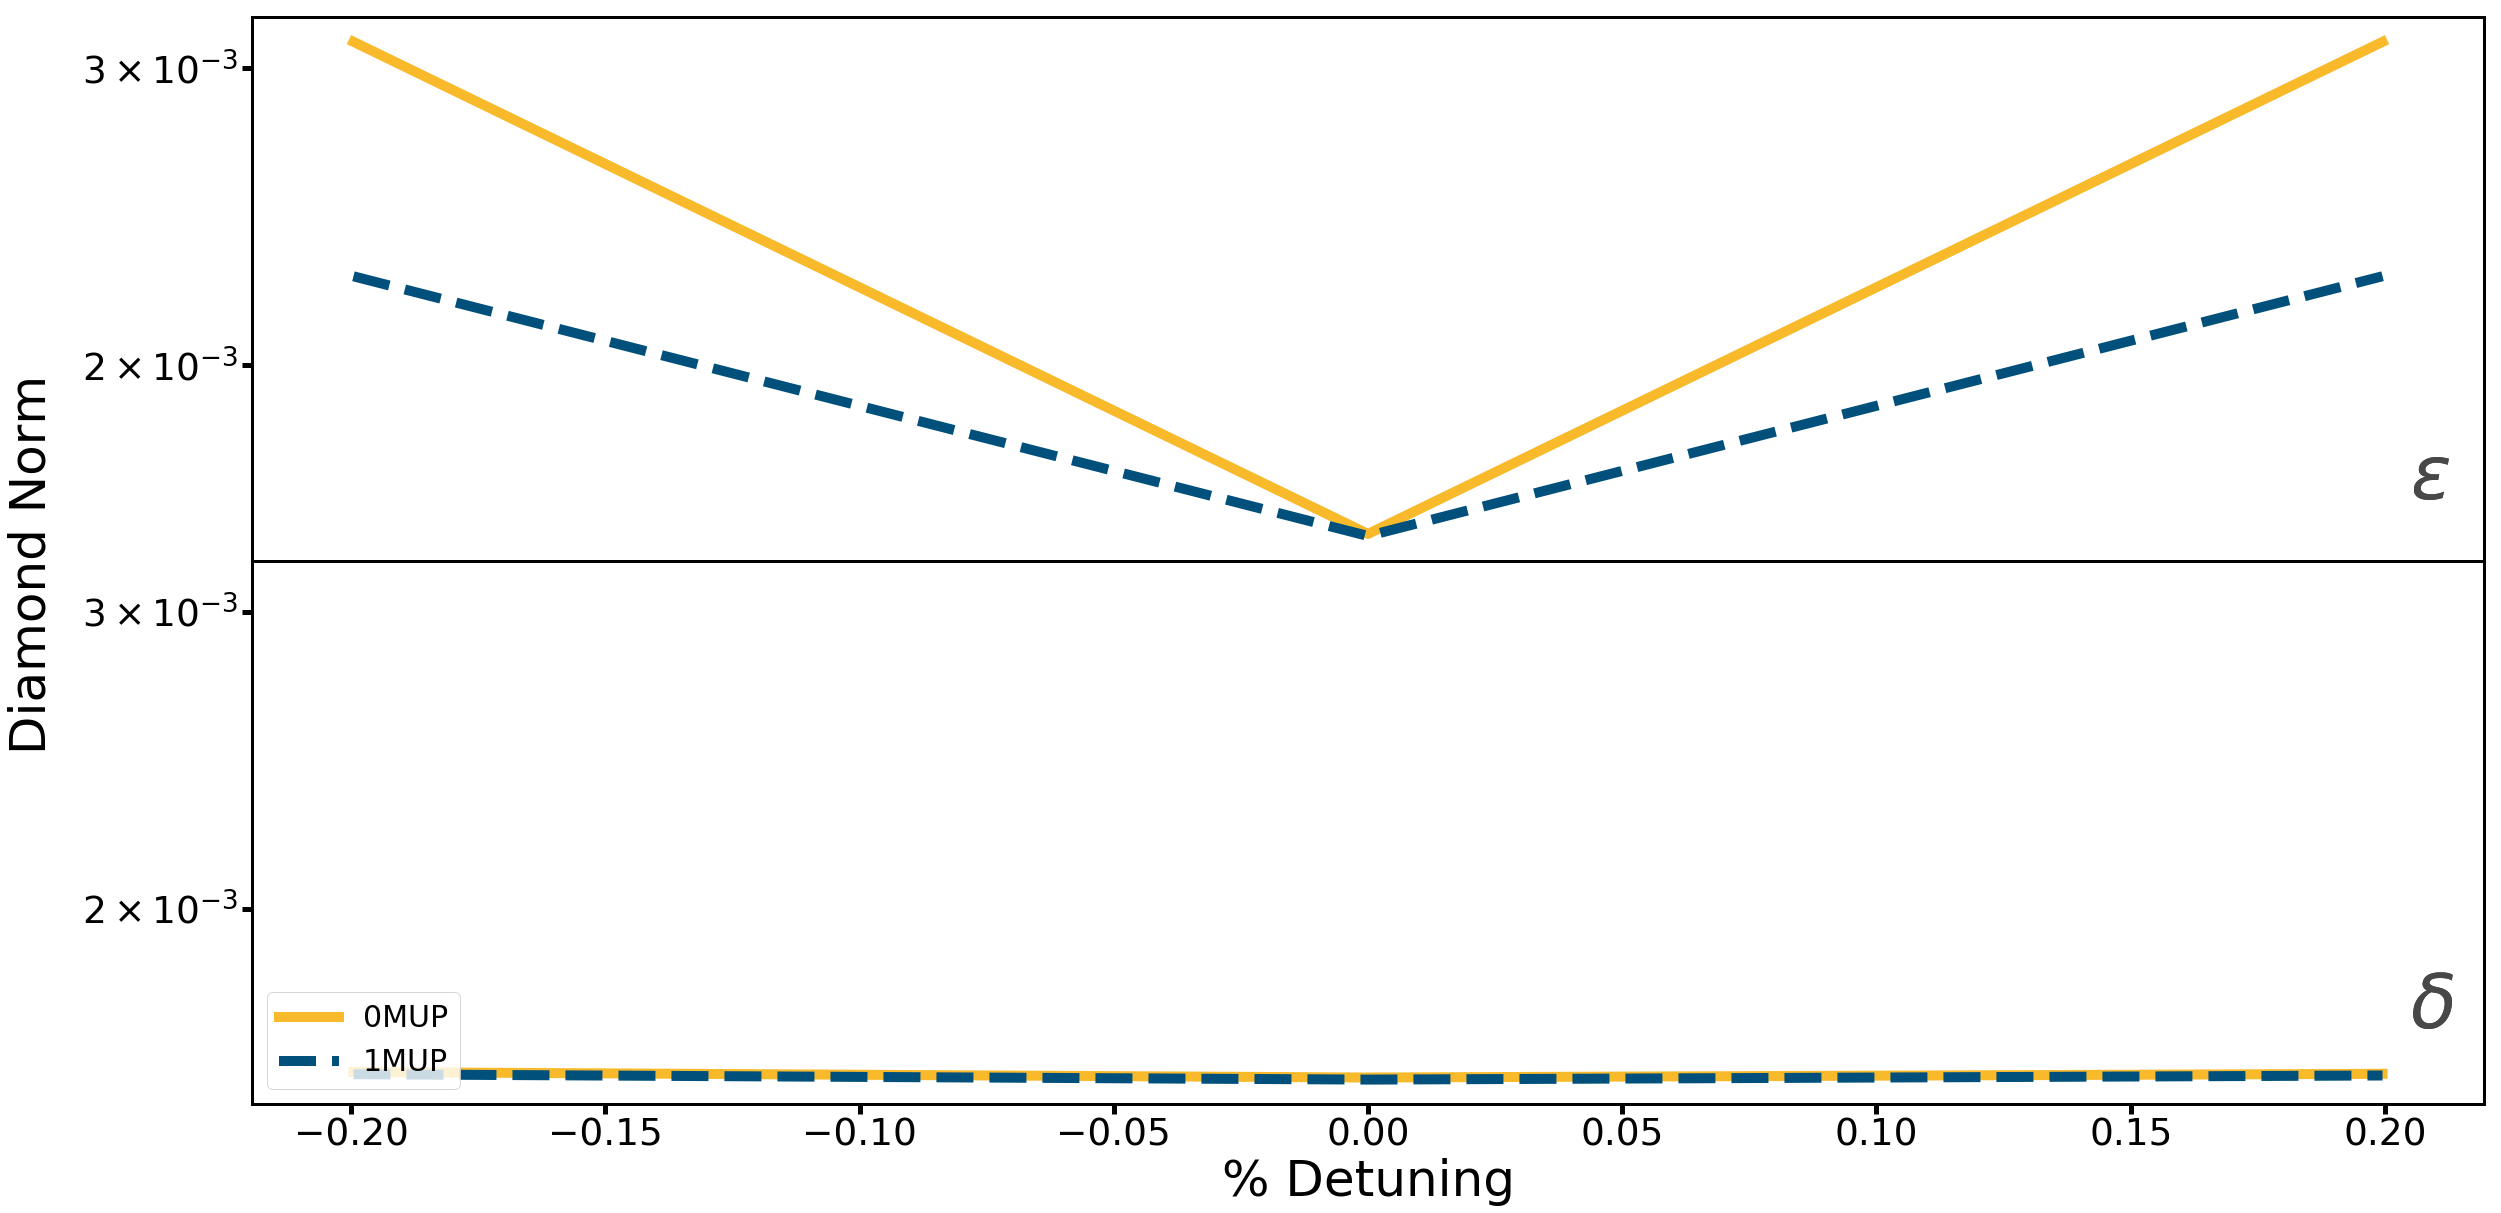
\includegraphics[width=\columnwidth]{2QRBC_no_member.png}
  \caption{Numerical results comparing a 0MQC to a 1MQC for a pair of tunable qubits, with a resonant exchange interaction. Shown with lower alpha values are example constituent controls. The 0MQC and 1MQC can be seen to outperform these controls by half of an order of magnitude at the origin. For all detuning values the 1MQC performs as well or better than the 0MQC. When there is $.2\%$ drift in the qubit frequency, the 1MQC outperforms members of the control famlies by almost an order of magnitude in diamond norm. Similarly, for $.2\%$ drift in the qubit control amplitude, we see that the 1MQC outperforms the the constituent controls by over half an order of magnitude.}
  \label{fig:2MQC}
\end{figure}






% ==============================================================================
% Section: Conclusion and Future Work
% ==============================================================================


\section{Conclusion and Future Work}
We have shown numerically that using MQCs can reduce coherent error on a quantum channel by more than an order of magnitude in diamond norm, over a wide range of quasi-static values of noise. In addition, we have demonstrated that these approximate controls can be generated through optimal control (GRAPE), and that the minimization problem is tractable.

Future directions for this work include demonstrating the routine experimentally on a two-qubit gate, moving the random gate selection from a precompilation step to runtime logic onboard the control electronics, investigating other optimization routines such as CRAB \cite{Caneva2011} and GOAT\cite{Machnes2018}, and using more sophisticated benchmarking routines such as GST\cite{BlumeKohout2017} to quantitatively investigate the performance of our method.

Another interesting area of research would be using model-free approaches. The numerical work in the paper assumes access to a model of the system, however an experimentalist may not have a model readily available to describe the system, e.g. in the presence of unknown on-chip crosstalk, or an uncalibrated transfer function of the system. Even if a model is available, it might be computationally inconvenient to simulate, i.e. for more than a few qubits.

In these situations, one approach would be to use \textit{in-situ} optimal control techniques \cite{Wu2018, Kelly2014, Ferrie2015} to generate candidate controls, and then use an optimizer like Nealder-Mead to perform the minimization. While performing a complete optimization in this way would require full process tomography, one could intead optimize via partial tomography. By selecting pre-- and post --rotations that correspond to measuring Pauli-moments of interest in the Hamiltonian, such as unwanted $Z\otimes Z$ crosstalk, one could perform optimization over fewer parameters.
% ==============================================================================
% Section: Acknowledgements
% ==============================================================================

\section{Acknowledgements}
\label{sec:acknowledgements}
Sandia National Laboratories is a multimission laboratory managed and operated by National Technology and Engineering Solutions of Sandia, LLC, a wholly owned subsidiary of Honeywell International, Inc., for the U.S. Department of Energy's National Nuclear Security Administration under contract DE-NA0003525.
\bibliography{decorrelation.bib}


\newpage
\onecolumngrid
% ==============================================================================
% Section: Appendix
% ==============================================================================
\section{Appendix}
\label{sec:appendix}
\subsection{Robust Mixing Lemma}
We begin by generalizing Lemma 2 from \cite{Campbell2017}. If all of our error Hamiltonians $\{H_j\}$ have bounded error, that is:
\begin{equation}
||H_j||\leq c
\end{equation}
Then we may consider the derivative of any mixture of unitaries as:
%\begin{equation}
%\deriv\sum_j \omega_je^{iH_j} = \deriv(\id + (\sum_ji%\omega_jH_j) + \sum \omega_j\sum_{n=2}^{\infty}%\frac{(iH_j)^n}{n!}))
%\end{equation}
\begin{equation}
\deriv\sum_j \omega_je^{iH_j} = \sum_j\omega_ji\deriv (H_j)e^{iH_j}
\end{equation}
By assumption, the derivatives of the first order term sum to zero, and so we see by A3 in \cite{Campbell2017} that
\begin{equation}
||\deriv\sum_j\omega_je^{iH_j}|| \leq \sum_j\omega_j||i\deriv (H_j)(iH_j + \sum_{n=2}^{\infty}\frac{(iH_j)^n}{n!})|| \leq \sum_j\omega_j(c^2 + \frac{c^2}{2}) \leq c^2 + \frac{c^3}{2}
\end{equation}
Where we have used the fact that $||AB|| \leq ||A||||B||$ with $||\cdot||$ being the $\infty$-norm.
Additionally, 
\begin{align}
||\deriv e^{iH_j}|| &= ||\deriv(iH_j)e^{iH_j}|| \\
&\leq ||\deriv(iH_j)|| + ||\deriv(iH_j)H_j|| +  ||\deriv(iH_j)\sum^{\infty}_{n=2}\frac{1}{(n)!}(iH_j)^n|| \\
&\leq ||\deriv(iH_j)|| + ||\deriv(iH_j)||\cdot||H_j|| +  ||\deriv(iH_j)||\cdot||\sum^{\infty}_{n=2}\frac{1}{(n)!}(iH_j)^n||\\
&\leq c + c^2 + \frac{c^3}{2}
\end{align}
And so we see that Lemma 2 generalizes. We will use the above to upper bound the 1-norm (and hence diamond norm) in the following.

Next we generalize the Mixing Lemma from \cite{Campbell2017}. We must assume that the 1-norm is uniformly differentiable. In that case, we see that:

\begin{align}
&= \deriv\sup|\mathcal{I}\otimes\mathcal{I}-\error(\vec{\delta})\otimes\mathcal{I}|_1 \\
&= \sup\deriv|\mathcal{I}\otimes\mathcal{I}-\error(\vec{\delta})\otimes\mathcal{I}|_1 \\
&\leq \sup|\deriv(\mathcal{I}\otimes\mathcal{I}-\error(\vec{\delta})\otimes\mathcal{I})|_1 \\
\end{align}
And so we see it is sufficient to upperbound:
\begin{equation}
|\deriv(\mathcal{I}\otimes\mathcal{I}-\error(\vec{\delta})\otimes\mathcal{I})|_1
\end{equation}
From Equation 18 in \cite{Campbell2017}:
\begin{align}
&(\mathcal{V}\circ\mathcal{E} - \id)(X) = \sum_j \omega_j(\tilde{\delta}_jX + X\tilde{\delta}_j^{\dagger} + \tilde{\delta}_jX\delta_j^{\dagger})\\
&\deriv(\mathcal{V}\circ\mathcal{E} - \id)(X) = \sum_j \omega_j(\deriv\tilde{\delta}_jX + X\deriv\tilde{\delta}_j^{\dagger} + \deriv\tilde{\delta}_jX\delta_j^{\dagger} + \tilde{\delta}_jX\deriv\delta_j^{\dagger})\\
\end{align}
Thus, by H\"older's inequality we find:
\begin{align}
&||\deriv(\mathcal{V}\circ\mathcal{E} - \id)(X)||_1\leq||\sum_j \omega_j\deriv\tilde{\delta}_j|| + ||\sum_j\omega_j\deriv\tilde{\delta}_j^{\dagger}|| + \sum_j\omega_j|| \deriv\tilde{\delta}_j||\cdot||\delta_j^{\dagger}|| + \sum_j\omega_j||\tilde{\delta}_j||\cdot||\deriv\delta_j^{\dagger}||
\end{align}
By assumption, all of these terms are neglible, and therefore we find:
\begin{align}
||\deriv(\mathcal{V}\circ\mathcal{E} - \id)(X)||_1\leq 2a^2 + 2b^2
\end{align}
And so we see that the mixing lemma extends to first order. In a similar way, it can be extended to arbitary order, and thus if we can find constructions that satisfy the generalized Lemma 2, we can use the Robust Mixing Lemma to conclude that there exists a weighting with linearly supressed diamond norm.
\end{document}